\documentclass[conference]{IEEEtran}
\IEEEoverridecommandlockouts{}
\usepackage{cite}
\usepackage{amsmath,amssymb,amsfonts}
\usepackage{graphicx}
\usepackage{textcomp}
\usepackage{xcolor}
\usepackage{subfig}
\usepackage[justification=centering]{caption}
\def\BibTeX{{\rm B\kern-.05em{\sc i\kern-.025em b}\kern-.08em
    T\kern-.1667em\lower.7ex\hbox{E}\kern-.125emX}}
\begin{document}

\title{Incredibly Realistic, Engaging, Real-World, Physics-Based, Flying Mini Cooper Simulator\\
}

\author{
Braden Wells\textsuperscript{1},
Brady Kruse\textsuperscript{1}
\\
Mississippi State University
\\
\small{braden@yougottabekidding.me, bradyakruse@gmail.com}

\thanks{\textsuperscript{1}These authors contributed equally to this project.}
}

\maketitle

\begin{abstract}
This project aimed to be a final culmination of all of the different graphics components learned over the past semester. Thus, we created a procedurally generated, infinite, skeleton world that can be flown over and explored through a camera following the infamous Mini Cooper model that we have used throughout the class. This creation involved several steps: loading and texturing the object files, performing linear algebra calculations to get correct perspective and movement through the virtual space, using random gradient equations to generate the world, and calculating proper lighting. The primary "new" component of the project is the tessellation shader used to generate the line-world. As such, since Regl does not support tessellation, we also had to port our learning into ModernGL--a Python library used for rendering. The following report is organized as follows: Section I details our initial plan, Section II explains the implementation of the project and issues we encountered, Section III serves as a conclusion, telling the current state of the project, its downfalls, and future potential.
\end{abstract}

\section{Project Plan}
{Computer graphics and game design often go hand in hand, so we wanted to create some form of interactive program that can be controlled. As stated before, we decided to create a flying simulator for the Mini Cooper model through a barebones world. With this, we could have both an interesting and engaging project, while also enjoying the whimsy of making a car fly.}
\\
\indent{The world serves as a backdrop for the rest of the program, so much work was done in planning how it was to be implemented. To save graphic resources (and to obtain a very aesthetic, science-fiction feel), we opted to make the world a skeleton framework, composed of lines and simple shapes rather than actual texture. We also planned to take full advantage of the "time" capability that OpenGL provides, using the time variable in tandem with trigonometry to cycle through colors as the program runs. Most importantly, the world needed to be infinite and procedurally generated, so that, instead of a flat grid, it has terrain in the form of hills and dips. The terrain should also be randomized so that one doesn't simply loop through the same, hard-coded terrains. Also, because of the infinite nature of the world, we would have to account for view length and preserving where one currently is (and the texture around that location), so that one could theoretically retrace their steps instead of the world being constantly and dynamically randomized as one moves through it. Per Dr. TJ's suggestion, the actual calculation of the world need take place in a tessellation shader rather than a vertex shader so that the world may be composed of subprimitives and therefore higher quality.}
\\
\indent {Moving to the objects, we planned to import the Mini Cooper model and use it as a controllable vehicle (in the most literal and metaphorical sense of the word) through the world. We also decided to use zebra model as an alternative to the car for absolutely no discernible purpose. The movable objects would require two parts:
\begin{itemize}
    \item Importing the .obj files
    \item Making the objects movable.
\end{itemize}
Importing the .obj files, we initially believed, would require a converter for the current Mini Cooper files. We would also need to learn how to import and render .obj files in ModernGL (to be explained more thoroughly later) to proper scale and texture.}
\\
\indent{Making the objects movable would be considerably more difficult, requiring the creation of a movable camera (and all necessary matrix calculations to do so) and then locking the objects in place in front of the camera. The movement would involve movement along all 3 axes, as well as rotation. This would also require a number of other minute things such as keybinding, key-listening, simultaneous rendering, etc.}
\\  
\indent {Finally, and initially more of a "if-we-have-time", we planned to implement lighting on the object. The grid world would, as previously mentioned, cycle between colors, and to complete the science-fiction aesthetic, we also hoped to light the object as it flew over the world. Logically, the light would need to get brighter and more intense as the object lowers itself closer to the world. We planned to implement full Phong lighting, complete with specular lighting (the zebra would be shiny for, again, no reason).}
\\
\indent {These four components primarily made up the full project, although there were several complications and workarounds along the way. These will be detailed in the following section.}
\\
\indent{As part of the planning phase, we also spent time determining what tools to use. 
\begin{enumerate}
    \item Since Regl does not support tessellation, we had to find an OpenGL binding that does, which we discovered in the Python-based ModernGL \cite{b1}. ModernGL is poorly documented and not widely used, although it did provide an extensive collection of demos (see Figure \ref{fig:ModernGLDemo}, from which we often pulled code snippets.
    \item To obtain the random world, we found an equation known as Perlin Noise: a randomized gradient (so that, based on inputs, the random output changes gradually rather than suddenly). Luckily, glsl libraries already existed for implementing it \cite{b2}.
    \item Finally, and perhaps most importantly, we desired a very high-quality and free zebra model, which we found in the form of the low-poly Figure \ref{fig:ShittyZebra} \cite{b3}
\end{enumerate}}
\begin{figure}[h]
    \centering
    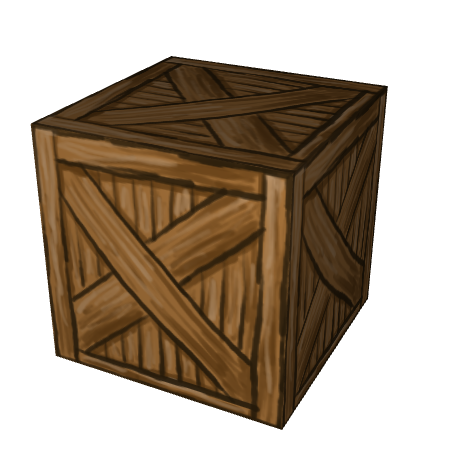
\includegraphics[width=0.2\textwidth, height=3cm]{Images/ModernGLDemo.png}
    \caption{Demo of ModernGL}
    \label{fig:ModernGLDemo}
\end{figure}

\begin{figure}[h]
    \centering
    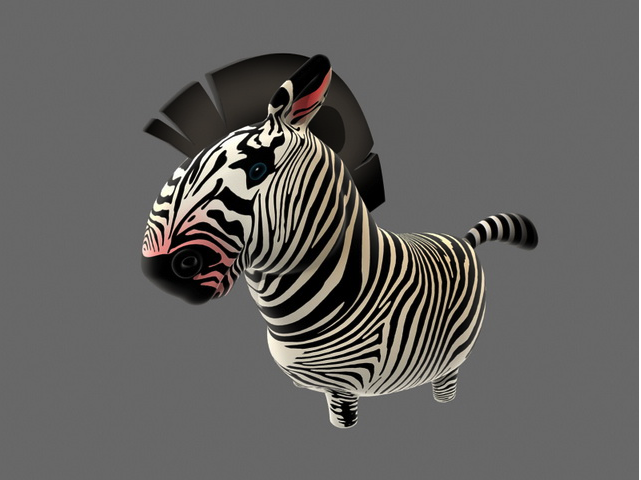
\includegraphics[width=0.2\textwidth, height=3cm]{Images/ShittyZebra.png}
    \caption{Low-Poly Zebra Model}
    \label{fig:ShittyZebra}
\end{figure}

\section{Implementation}
The implementation process took place over the period of about 2 weeks, with plenty of trial and error along the way, mainly due to ModernGL's shockingly terrible documentation.
\subsection{Creating The World}
As the world serves as a backdrop for the entire rest of the project, we decided to set about creating it first. Luckily, ModernGL provided a textured world (see Figure \ref{fig:TexturedWorld}) that we used as a template (although, now, I believe almost every line of code has been changed). The world achieved its terrain through modification of the Z value based on a provided Perlin Noise .jpg, then modified color based on the photo as well.
\begin{figure}[h]
    \centering
    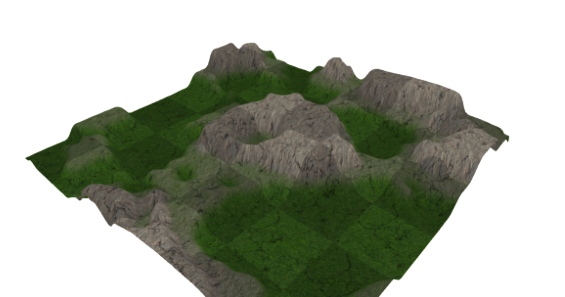
\includegraphics[width=0.4\textwidth, height=4cm]{Images/TexturedWorld.png}
    \caption{Initial World}
    \label{fig:TexturedWorld}
\end{figure}
\\
\indent {Our edits began by stripping the textured world to a wireframe model, as seen in Figure \ref{fig:StrippedWorld}. We were unsure about how to do this, as the vertexes and indices passed into the program were designed for triangles, not lines or squares. However, one of the more handy parts about ModernGL is the ability to change render type by simply modifying the string passed into the render call. 
\begin{figure}[h]
    \centering
    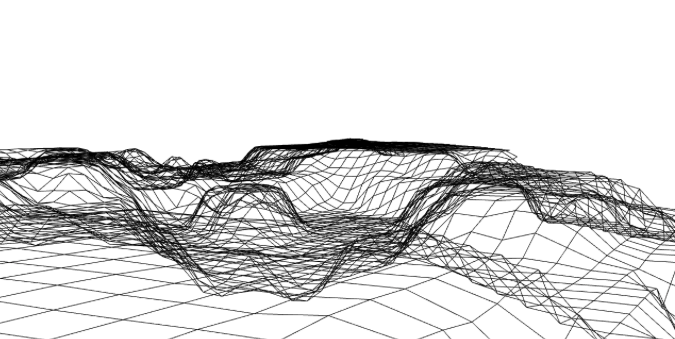
\includegraphics[width=0.4\textwidth, height=4cm]{Images/StrippedWorld.png}
    \caption{Stripped World}
    \label{fig:StrippedWorld}
\end{figure}
Once we achieved this, we then modified the fragment shader to loop through colors, directly manipulating color channels. This took some time, mainly because we had absolutely no idea how to actually pass uniforms in through ModernGL (it is not at all intuitive like Regl). Nonetheless, once we finally were able to pass in the time variable, we very quickly achieved Figure \ref{fig:ColorfulWorld}.}
\\
\begin{figure}[h]
    \centering
    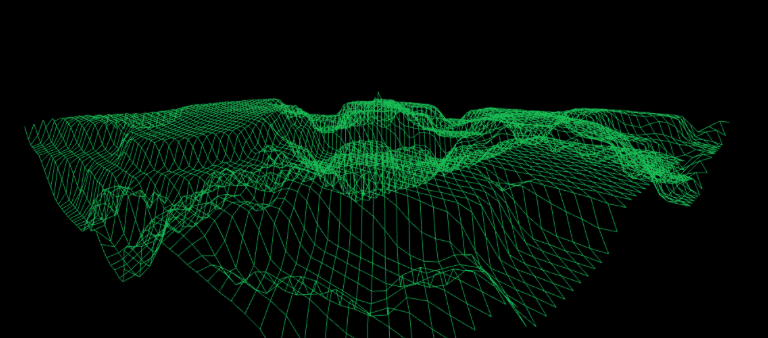
\includegraphics[width=0.4\textwidth, height=4cm]{Images/ColorfulWorld.png}
    \caption{A Still From the Dynamically Colored World}
    \label{fig:ColorfulWorld}
\end{figure}

\indent {Now that we had a stripped down, colored world, we next had to figure out how to implement the Perlin Noise equations in \cite{b2}. This ended up being quite easy--the equations are rather intuitive--so it took almost no time at all to modify them so that the x and y of each vertex is passed in, then a gradient z value is kicked out. This created a random world, but a finite one; once the camera left the box defined by {{-1,1}, {-1,1}}, the camera would fall off the world.}
\\
\indent{We spent an embarrassing amount of time tinkering with how to make the world infinite, but also retaining previous environment (so that going backwards wouldn't create new z values for areas where the camera has already been). We spent time thinking about some kind of offset system, so the world actually moves instead of the camera, or a slice system, where the world only renders once the camera leaves its previous "slice." The answer ended up being incredibly simple: Perlin Noise works on a seed system, the coordinate (1,1) will always create the same z value. So, since Perlin Noise already worked like this, all we had to do was generate the world based on the camera coordinates rather than the vertex coordinates, effectively creating an infinite, retained world. The world now looked something like Figure \ref{fig:InfiniteWorld}}
\begin{figure}[h]
    \centering
    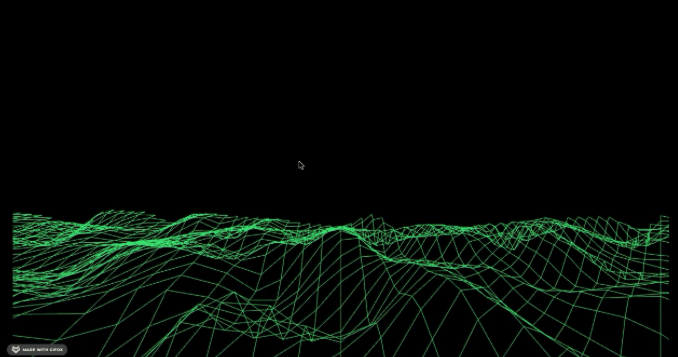
\includegraphics[width=0.4\textwidth, height=4cm]{Images/InfiniteWorld.png}
    \caption{An Infinitely Perlin World}
    \label{fig:InfiniteWorld}
\end{figure}
\\
\indent{Interestingly enough, we had an issue we deemed "shimmering." The ground seemed to wave as the camera moved across the environment, and we nearly tore our hair out wondering why. Turns out, the way the ModernGL "wire strip" parameter worked was by stretching vertexes over the Z values (so, as we moved forward, the squares would slowly stretch and shrink off screen). We found a hacky-fix for the issue by increasing the polygon count tenfold, from 64 to 512 (see Figure \ref{fig:HigherPolygonCountWorld}. Then, as all college students would do, we set it to 10,000, and managed to see a terribly artifacted, horribly bright world that ran at a whopping 1 frame per second before overheating my Mac and crashing. This was our progress at our presentation.}
\begin{figure}[h]
    \centering
    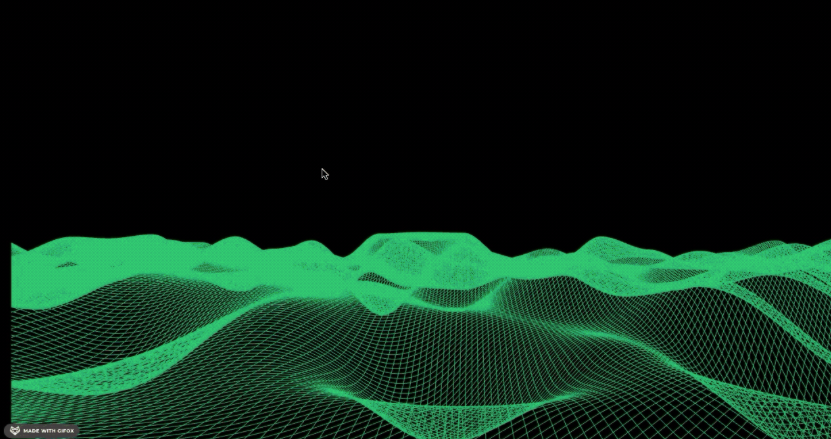
\includegraphics[width=0.4\textwidth, height=4cm]{Images/HigherPolygonWorld.png}
    \caption{Increased Polygon Count to 512}
    \label{fig:HigherPolygonCountWorld}
\end{figure}
\\
\indent {Up until this point, all of the calculations for creating the world had been done in the vertex shader, which likely contributed to the reduced run speed at higher polygon counts. We now decided to move our work into the tessellation shader which, surpringly enough, are equally poorly documented in ModernGL. Braden spent several hours trying to figure out the syntax for tessellation shaders before we finally decided to email Dr. TJ. He provided a fantastic little example that we were able to borrow and modify to fit our purposes \cite{b4}.}
\\
\indent{The tessellation shader is made up of two different parts: the control shader and the evaluation shader. The control shader serves to decide to what extent we will perform tessellation. We set the control levels to a scale value (similar to how we could increase polygon counts earlier), which is passed in as a uniform. The control shader passes through vertex positions and outputs a layout of quads to the evaluation shader. The evaluation shader is almost a copy / paste of our previous vertex shader that implemented Perlin Noise. The evaluation shader then outputs the glPosition that is rendered. This is the current status of the world.}

\subsection{Camera}
While creating the world, we simultaneously worked on the camera, and performed all necessary linear algebra chicanery to do so (or rather, found libraries to do it for us, as all good computer scientists should).
\\
\indent {Once again, ModernGL had a example that involved a moving camera and all necessary keybinds, which we copied and modified into our project. Mainly, the example had a pre-created camera class, saving us the trouble of writing a few dozen lines of code. After plenty of modification and linear algebra review, we had a movable camera, set up from 3 parts, camera front, camera position, and camera target. In that set up, the location of the user is at the camera position, and target only changes through rotation either up or down (which involved the use of quaternions designed for rotation about an axis.) Most of our issues came from rotation and understanding how the axes were set up, most importantly, negative Z is "up" instead of down. A majority of our programming issues came from the linear algebra involved with the camera, mainly small things such as projections not being calculated properly or matrix multiplication out of order.}
\\
\indent{We then did some minor modifications to aid in program usability. We changed some class variables from private to public, so that we could pass them into the shaders (such as camera position for Perlin Noise), changing camera speed, and creating a key to allow for automated roaming around the map, good for demonstration purposes. All of this had been done before our presentation}

\subsection{Objects}
Importing of objects ended up being likely the most difficult task that we encountered. Most of our issues came from ModernGL syntax, but we also had to modify our program in terms of camera position and perspective. We also used the objects as justification for lighting, and spent time figuring out how to calculate light based on distance. This has all been completed since our presentation.
\\
\indent{For a sample object, we decided to use the simple zebra .obj file, then saved the more complicated Mini Cooper for last. ModernGL handles objects through assigning them to a vao variable, so, we assigned our world to vao and our zebra to vao2, allowing us to render them both in order. We encountered plenty of strange errors when trying to load the zebra and the zebra texture into the program, before eventually realizing that we were passing the zebra into the same vertex and fragment shader as the grid. Thus, we created a seperate zebra.glsl file that handles the zebra rendering. Once this was set up, loading the object and the texture was fairly straightforward after some minor scaling and positioning. The first time we saw the zebra ended up being rather humorous, as shown in Figure \ref{fig:DrowningZebra}.}
\begin{figure}[h!]
    \centering
    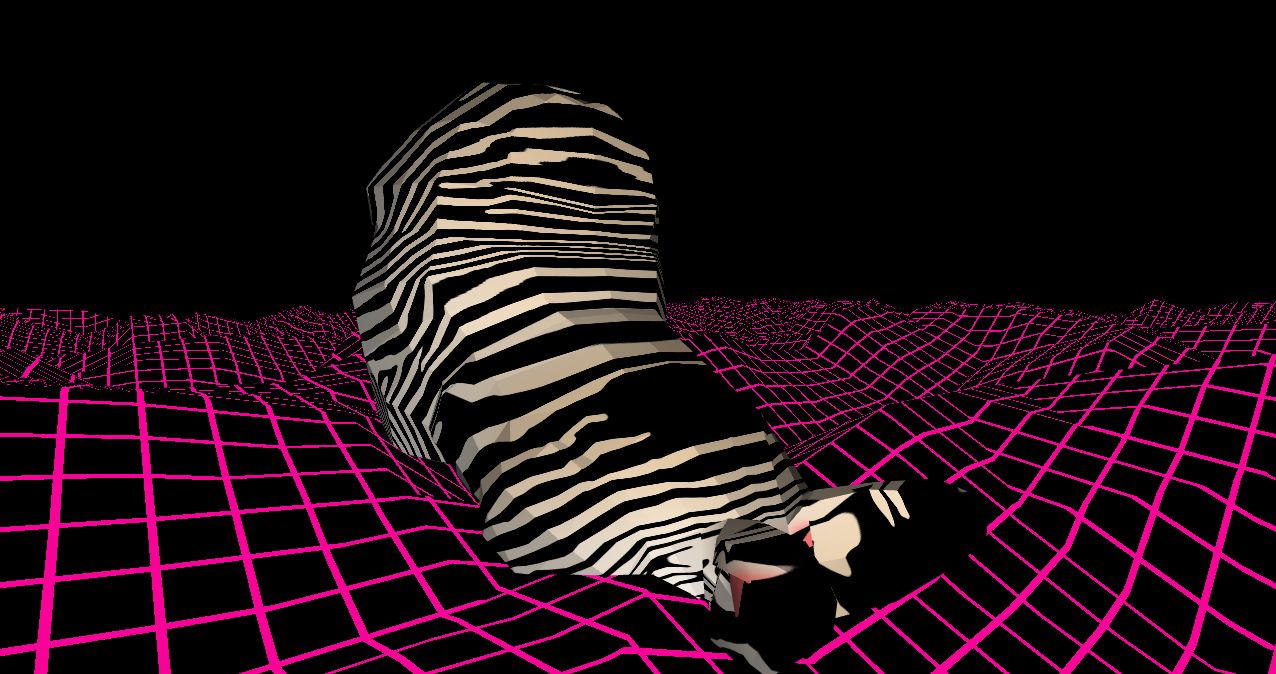
\includegraphics[width=0.4\textwidth, height=4cm]{Images/drowning.png}
    \caption{A Drowning Zebra}
    \label{fig:DrowningZebra}
\end{figure}
\\
\indent{Now that we had an object loaded, we needed to lock it in front of the camera and rotate along with the camera. The first thing we did was change our rotation style from a matrix based on the Z-axis to an angle (up until this point the camera point had been rotated about the origin) We then oriented the zebra front to be aligned with the camera front and the zebra position to move with the camera position. This made the zebra move with the camera, but instead would rotate around the zebra when we actually desired the zebra to rotate with the camera, as shown in Figure \ref{fig:BadRotation}.}
\begin{figure}[h]
    \centering
    \subfloat[Placed behind the zebra]{{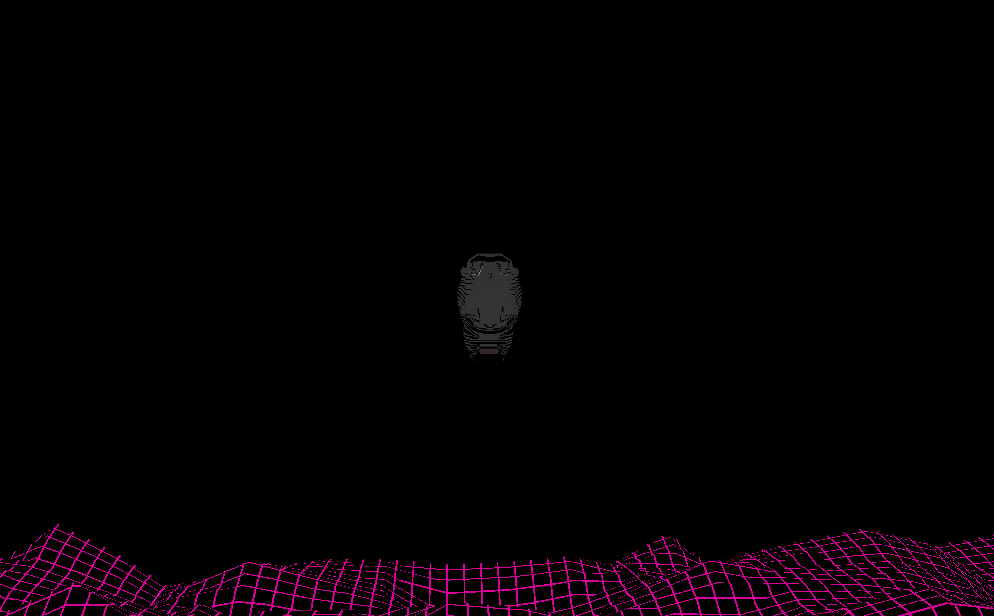
\includegraphics[width=5cm]{Images/BadRotation.png} }}%
    \qquad
    \subfloat[Rotated around the zebra]{{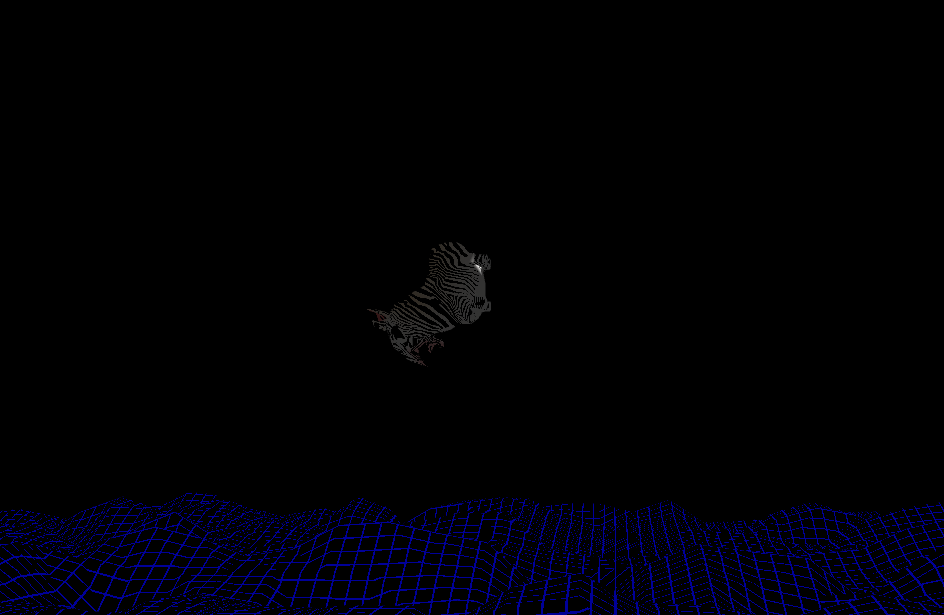
\includegraphics[width=5cm]{Images/BadRotation2.png} }}%
    \caption{Bad Rotation Around the Zebra}%
    \label{fig:BadRotation}
\end{figure}
\\
\indent{We fixed this by changing how the camera works. Until this point, camera target had been set to whatever direction the camera is facing, and camera position handled movement. Now, we did the inverse of this: camera target is now set to the camera position, and the zebra is rendered at the camera position. We also kept track of rotation and applied it to the camera position and zebra, so that, when one rotates, they both do, and the target follows them together. This is the method typically used in game design, so it worked well with our program. We also made sure to keep track of the z location (so that the zebra can float up and down) and normalize vectors as appropriate, so the distance between the camera target and the zebra did not change. We ended up removing the rotate up capability, as we couldn't think of a good way to implement it. Should the zebra rotate up, or the camera rotate underneath the zebra? Either way, it would have required a lot of coding that we did not have time for, especially for a largely unnecessarily capability. Our status at this point can be seen in Figure \ref{fig:ProperRotation}}
\begin{figure}[h]
    \centering
    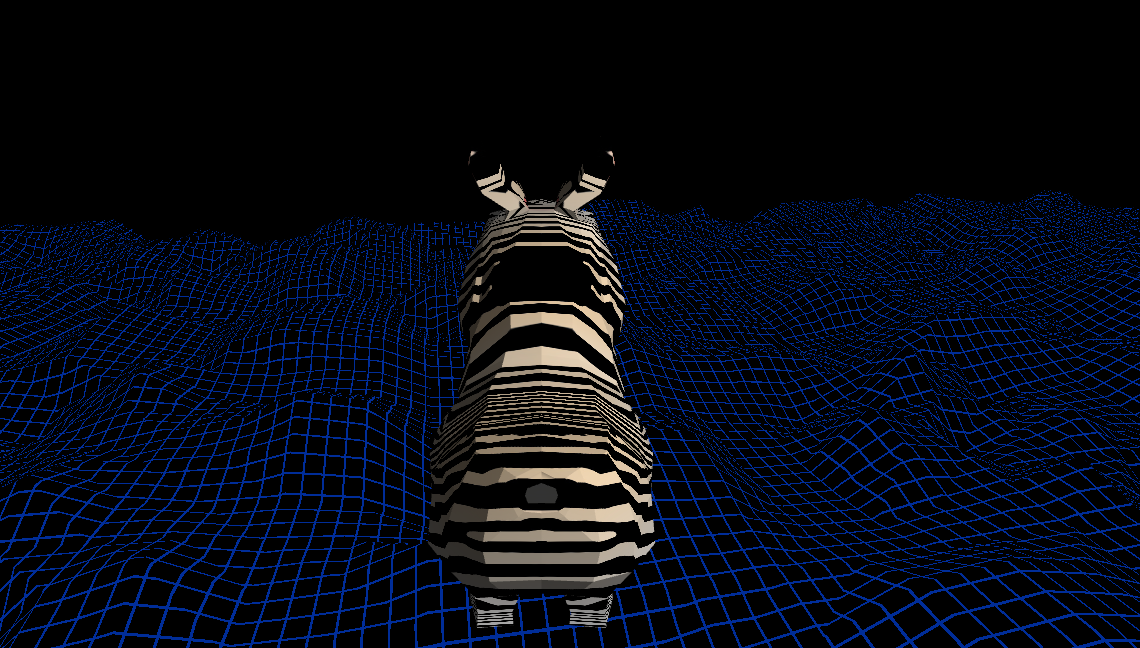
\includegraphics[width=0.4\textwidth, height=4cm]{Images/ProperRotation.png}
    \caption{Proper Rotation of the Zebra}
    \label{fig:ProperRotation}
\end{figure}
\\
\indent{We now moved to importing the Mini Cooper model \cite{b5}, which ended up being rather easy since we already had the necessary calculations in place. We had some minor difficulty with scaling (see Figure \ref{fig:MiniCooperMessups} and the normal texturing issues (placing texture on the windshields and such), but were able to import it after some debugging. We also created a keybind to switch between objects.}
\begin{figure}[h]
    \centering
    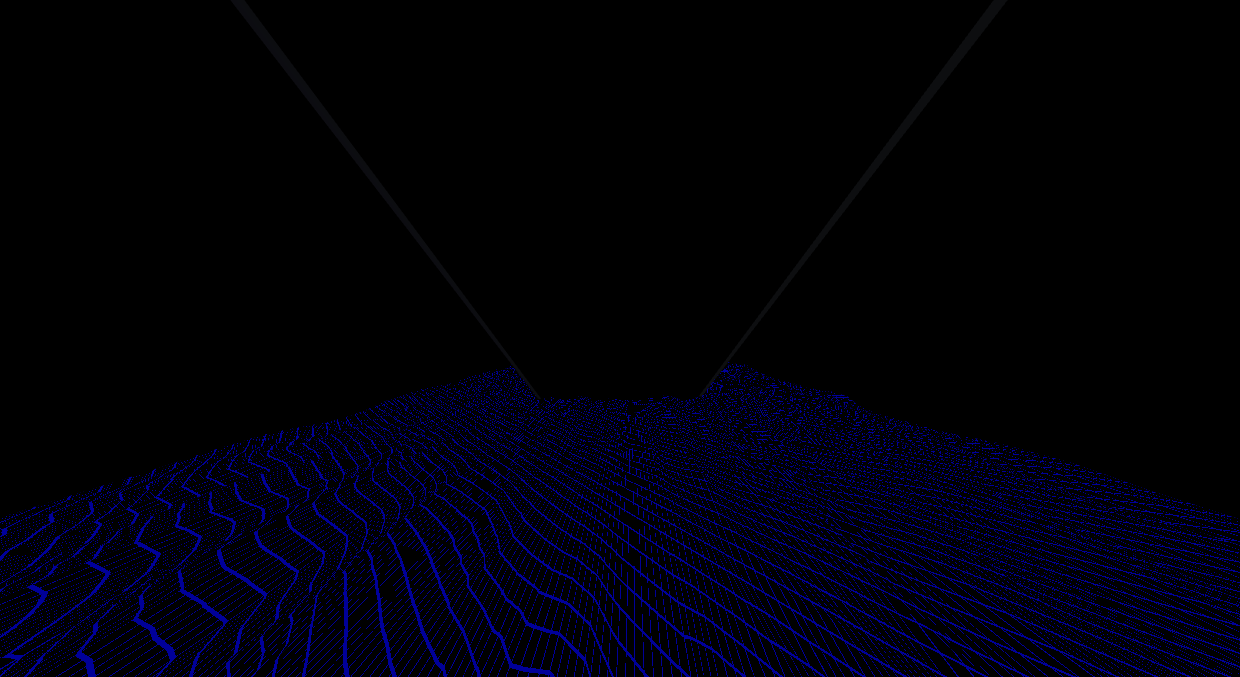
\includegraphics[width=0.4\textwidth, height=4cm]{Images/bigboy.png}
    \caption{A Very Obnoxiously Large Mini Cooper}
    \label{fig:MiniCooperMessups}
\end{figure}
\\
\subsection{Lighting}
Now that all of our objects were loaded, we decided to implement some very basic lighting effects. We considered doing specular lighting, but realized that we would have to calculate normals for our zebra object, and, since it was, in fact, finals week, we elected to stick to ambient and diffuse.
\\
\indent{We began with diffuse lighting by importing the time variable into our object glsl file, then setting up the same trig functions as we have in the world fragment shader so that the light is the same color. We offset the light slightly to the left of the object and provided a gray ambient light to produce the effect in Figure \ref{fig:BasicLighting}.}
\begin{figure}[h]
    \centering
    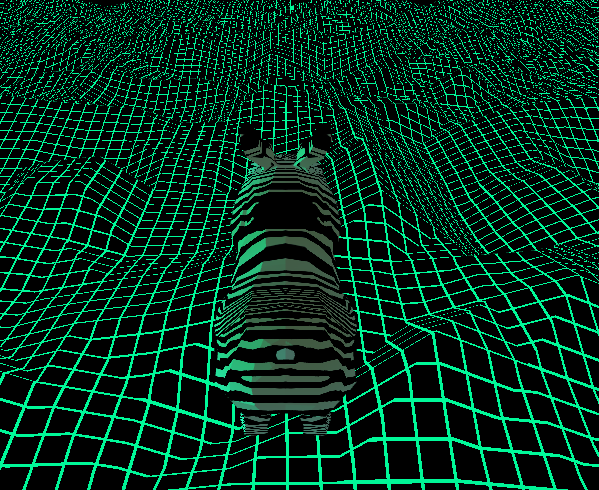
\includegraphics[width=0.4\textwidth, height=4cm]{Images/BasicLighting.png}
    \caption{A Basic Lighting Model Local to the Object}
    \label{fig:BasicLighting}
\end{figure}
\\
\indent{Something not covered in Assignment 5 was light strength based on distance. We decided that this would neat to implement, so that as the zebra got lower and closer the ground, the light got stronger, and vice versa. Our theory was to simply take the object's z value, the ground's z value, subtract them, then scale the absolute value as necessary Again, we spent embarrassingly long on this, as it took a few hours to realize we were subtracting two unique variables that both held the object's z value because of some accidental redundant assignment. Once we finally realized this, we get the current effect as seen in Figure \ref{fig:CurrentLighting}.}
\begin{figure}[h]
    \centering
    \subfloat[The zebra far away from the grid]{{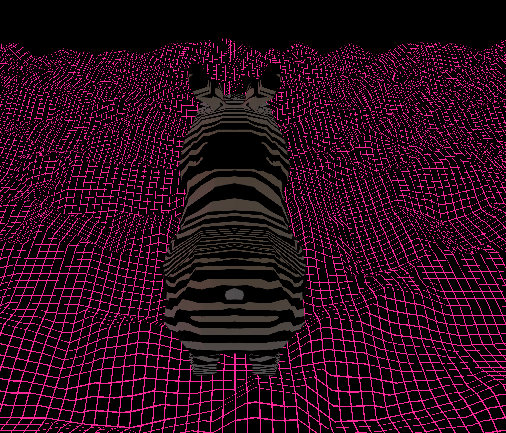
\includegraphics[width=5cm]{Images/FarLight.png} }}%
    \qquad
    \subfloat[The zebra close to the grid]{{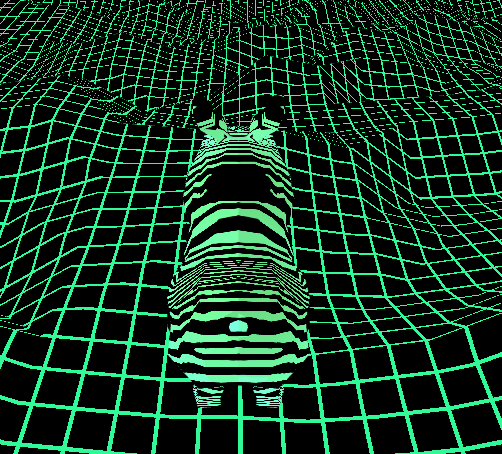
\includegraphics[width=5cm]{Images/CloseLight.png} }}%
    \caption{Current Lighting Model}%
    \label{fig:CurrentLighting}
\end{figure}
\\
\section{Conclusion and Future Works}
As previously stated, this is the current status of our project:
\begin{itemize}
    \item{A procedurally generated, non-textured, infinite landscape}
    \item{A working camera that tracks objects properly}
    \item{Two scaled and textured, movable objects}
    \item{A very simple distance-based diffuse / ambient lighting model.}
\end{itemize}
Through the implementation of these four things, we have demonstrated a general overview of all the methods taught in this class through ModernGL.
\indent{As with all computer programs, there is always significant room for improvement. For good practice, we will likely implement these for fun in the future.
\begin{itemize}
    \item {The lighting model is painfully basic. There is definite potential for a really beautiful specular effect that wouldn't be too incredibly complex to implement}
    \item {The camera does not support up or down rotation. This may or may not be very useful or relevant, but, nonetheless, could be implemented.}
    \item {There is significant artifacting occurring when the camera gets too far away from the grid.}
    \item {Upon starting and stopping movement, the color on the grid dims for a millisecond. We think this may be correlated with the artifacting occurring.}
    \item {We attempted to implement ground snapping (adding collision with the ground so the object cannot float through the grid) by replicating the glsl noise function in Python, but, for some reason, had small differences in our values. We think it has something to do with how Python handles floats. Instead, we simply made it impossible to go above 0 on the z-axis, so the object can slightly submerge in the grid.}
    \item {The black sky is nice, but a skybox could complete the sci-fi aesthetic we were going for, and also opens up opportunity for reflection (especially on the Mini Cooper with windshields and such)}.
    \item {We are unable to use alpha blending on the windshield of the Mini Cooper}
\end{itemize}}
\section*{Acknowledgment}
The project members wish to express their thanks to Dr. TJ for his help and for teaching a very difficult, yet thorough and fair, computer graphics class (along with putting up with our stupid memey chicanery)

\bibliography{biblio}
\bibliographystyle{ieeetr}

\end{document}
